\documentclass{article}
\usepackage[left=3cm,top=3cm,right=2cm,bottom=2cm]{geometry}
\usepackage{amssymb}
\usepackage{amsmath}
\usepackage{cancel}
\usepackage{xcolor}
\usepackage{enumitem}
\usepackage{graphicx}

\title{(Universidade de São Paulo)\\
Trabalho 01 - Temperaturas no Grafo de Manhattan}

\author{Métodos do Cálculo Numérico I -- SME0205\\
Docente: Antonio Castelo Filho\\[.2cm]
Julia Guazzelli Monteiro -- 15465383\\
Vinícius de Sá Ferreira -- 15491650}

\date{21 abr. 2025}

\begin{document}
    \maketitle
    
    \section{Modelagem do problema}

    Suponha $T: \mathbb{N} \times (\mathbb{R} \setminus \mathbb{R}^-) \to \mathbb{R}$ definida por $T(x,t) =$ \verb|temperatura no ponto |$x$\verb| ao tempo |$t$. Temos a equação do calor em 1D da seguinte forma
    \[\frac{\partial T(x,t)}{\partial t} = \alpha \frac{\partial^2 T(x,t)}{\partial x^2}\]
    onde $\alpha > 0$ é a difusão térmica. Assim podemos fazer a aproximação por série de Taylor para um $t_0$ fixo, ao redor de $x$
    \[T(x+1) = \sum_{j=0}^{+\infty} \frac{T^{(j)}(x) (\cancel{x}+1-\cancel{x})^j}{j!} = \sum_{j=0}^{+\infty} \frac{T^{(j)}(x)}{j!} = T(x) + T'(x) + \frac{T''(x)}{2} + \frac{T^{(3)}(x)}{6} + \frac{T^{(4)}(x)}{24} + \cdots\]
    \[T(x-1) = \sum_{j=0}^{+\infty} \frac{T^{(j)}(x) (\cancel{x}-1-\cancel{x})^j}{j!} = \sum_{j=0}^{+\infty} (-1)^j\frac{T^{(j)}(x)}{j!} = T(x) - T'(x) + \frac{T''(x)}{2} - \frac{T^{(3)}(x)}{6} + \frac{T^{(4)}(x)}{24} - \cdots\]
    \[T(x+1)+T(x-1) = 2T(x) + T''(x) + \frac{T^{(4)}(x)}{12} + \cdots\]
    \[ T''(x) = T(x+1)-2T(x)+T(x-1) - \frac{T^{(4)}(x)}{12} - \cdots\]
    \[\therefore T''(x) = T(x+1)-2T(x)+T(x-1) \color{gray}{- \mathcal{O}(1)}\]
    logo se definirmos $T_i(t) := T(t,i)$, teremos
    \[\frac{dT_i(t)}{dt} = \alpha (T_{i+1}(t)-2T_i(t)+T_{i-1}(t))\]

    Portanto, se tivermos $T(t) = \left[ \begin{array}{c}
        T_1(t)\\
        T_2(t)\\
        T_3(t)\\
        \vdots\\
        T_n(t)
    \end{array} \right]$, podemos reescrever a equação em função do Laplaciano $L$ do grafo, dado por $L = G-A$, com $G$ a matriz diagonal com o grau de arestas para cada vértice e $A$ a matriz de adjacência. Note que
    \[LT = \left( \left[ \begin{array}{ccccc}
        G_1 & 0 & 0 & \cdots & 0\\
        0 & G_2 & 0 & \cdots & 0\\
        0 & 0 & G_3 & \cdots & 0\\
        \vdots & \vdots & \vdots & \ddots & \vdots\\
        0 & 0 & 0 & \cdots & G_n
    \end{array} \right] - \left[ \begin{array}{ccccc}
        &&&&\\
        &&&&\\[.19cm]
        &&A&&\\
        &&&&\\[.19cm]
        &&&&\\
    \end{array} \right] \right)_{n \times n}\left[ \begin{array}{c}
        T_1\\
        T_2\\
        T_3\\
        \vdots\\
        T_n
    \end{array} \right]_{n \times 1} = \left[ \begin{array}{c}
        C_1\\
        C_2\\
        C_3\\
        \vdots\\
        C_n
    \end{array} \right]_{n \times 1}\]
    em que, para $i=1,2,3,\cdots,n$ teremos
    \[C_i = G_i T_i - \sum_{j \to i} T_j\]
    onde $j \to i$ indica os vizinhos de $i$, aqueles que estão conectados com $i$. No caso 1D, o grau de um ponto $i$ interno é de 2 e possui 2 pontos conexos, o sucessor e o antecessor, logo teremos a equação
    \[\frac{dT_i(t)}{dt} = \alpha (T_{i+1}(t)-2T_i(t)+T_{i-1}(t)) = -\alpha (2T_i(t) - T_{i-1}(t) - T_{i+1}(t)) = -\alpha (G_i T_i(t) - \sum_{j \to i} T_{j}(t)) = -\alpha (LT)_i\]

    Portanto, temos
    \[\frac{dT}{dt} = -\alpha LT\ (*)\]
    
    Uma forma de estender $T(t)$ para $\mathbb{R}$ é com $T(t) = e^{(-\alpha Lt)}T(0)$, onde $T(0) = T_0$. Assim
    \[\frac{dT}{dt} = \frac{d}{dt}[e^{(-\alpha Lt)}T(0)] = -\alpha L e^{(-\alpha Lt)}T(0) = -\alpha L (e^{(-\alpha Lt)}T(0)) = -\alpha L T(t)\]
    que satisfaz $(*)$. Por fim, se fizermos $\displaystyle{ \lim_{t \to +\infty} T(t) = T_\infty = \left[ \begin{array}{c}
        c\\
        c\\
        c\\
        \vdots\\
        c
    \end{array} \right] }$, $c \in \mathbb{R}$, logo $\dfrac{dT}{dt} = 0$ e a equação fica da seguinte forma
    \[\frac{dT}{dt} = -\alpha LT_\infty = \vec{0}\]
    \[LT_\infty = \vec{0}\]
    \[T_{i+1}(t)-2T_i(t)+T_{i-1}(t) = 0\]
    \[\therefore T_i(t) = \frac{T_{i-1}(t)+T_{i+1}(t)}{2}\]

    Agora, podemos adicionar condições de contorno, então teremos para $b$ o vetor com a temperatura em alguns pontos 
    \[\frac{dT}{dt} = -\alpha LT + b = 0\]
    \[\alpha LT = b\]

    Com a matriz de penalidades, ajustamos a contribuição resultando em

    \[(L+P)T = Pb\]

    \newpage

    \section{Métodos iterativos}

    \subsection{Gauss-Jacobi}
    Queremos resolver o sistema $Mx = c$, em que $M = (L+P)T$ e $c = Pb$. Assim, temos
    \[Mx = c\]
    \[(M-D+D)x = c\]
    \[(M-D)x + Dx = c\]
    \[(M-D)x^{(k)} + Dx^{(k+1)} = c\]
    \[Dx^{(k+1)} = (D-M)x^{(k)} + c\]
    \[x^{(k+1)} = D^{-1}(D-M)x^{(k)}+D^{-1}c\]
    \[x^{(k+1)} = (I-D^{-1}M)x^{(k)}+D^{-1}c\]
    \[x^{(k+1)} = Cx^{(k)} + g\]
    Como $D$ é a diagonal de $M$, o determinante é o produtório da diagonal e $M$ que é não-nulo, então $D$ é inversível. O método convergiu em $k = 1280$ iterações e demorou uma média de $3min$ para uma tolerância de $\pm 10^{-3}$.

    \subsection{Gauss-Seidel}
    Queremos resolver o sistema $Mx = c$, em que $M = (L+P)T$ e $c = Pb$. Assim, façamos $M = L+R$, onde $L$ é a matriz triangular inferior de $M$ e $R$, a triangular superior sem a diagonal, então
    \[Mx = c\]
    \[(L+R)x = c\]
    \[Lx + Rx = c\]
    \[Lx^{(k+1)} + Rx^{(k)} = c\]
    \[Lx^{(k+1)} = - Rx^{(k)} + c\]
    \[x^{(k+1)} = (-L^{-1}R)x^{(k)} + L^{-1}c\]
    \[x^{(k+1)} = Cx^{(k)} + g\]

    Como $L$ é triangular inferior, o determinante é o produtório da diagonal de $M$ que é não-nulo, então $L$ é inversível. O método convergiu em $k = 657$ iterações e demorou uma média de $2 min$ para uma tolerância de $\pm 10^{-3}$.

    \subsection{Gradientes conjugados}
    Queremos resolver o sistema $Mx = c$, em que $M = (L+P)T$ e $c = Pb$. Considere a função
    \[f(x) = \frac{1}{2}x^TMx - c^Tx\]
    onde $M$ é simétrica positiva definida (SPD). Note que
    \[f(x) = \frac{1}{2} \sum_{i=1}^{n}\sum_{j=1}^{n} m_{ij} x_{i} x_{j} - \sum_{i=1}^{n} c_{i} x_{i}\]
    \[\frac{\partial f(x)}{\partial x_k} = \frac{1}{2} \left( \sum_{i=1}^{n}\sum_{j=1}^{n} m_{ij} (x_{i} \delta_{ik} + x_{j} \delta_{jk}) \right) - c_k = \frac{1}{2} \left( \sum_{i=1}^{n} m_{ik} x_{i} + \sum_{j=1}^{n} m_{kj} x_{j} \right) - c_k\]
    \[= \frac{1}{\cancel{2}} \left( \cancel{2} \sum_{j=1}^{n} m_{kj} x_{j} \right) - c_k = \sum_{j=1}^{n} m_{kj} x_{j} - c_k\]
    \[\therefore \nabla f(x) = Mx - c\]

    \newpage

    Assim, queremos encontrar $x$ (que é único, porque $M$ é SPD) tal que $\nabla f(x) = 0 \iff Mx-c = 0 \iff Mx = c$.

    Começamos com um chute inicial $x_0$, então teremos um resíduo $r_0 = c - Mx_0 = -\nabla f(x_0)$. Teremos a direção inicial dada por $p_0 = r_0$, assim atualizamos
    \[x_1 = x_0 + \alpha p_0\]
    Temos que $r_1^T \cdot r_0 = 0$, porque são ortogonais, e $r_1 = c-Mx_1$, então
    \[r_1^T \cdot r_0 = 0\]
    \[(c-Mx_1)^T \cdot r_0 = 0\]
    \[[c-M(x_0 + \alpha p_0)]^T \cdot r_0 = 0\]
    \[(c-Mx_0)^T \cdot r_0 - \alpha(Mp_0)^T \cdot r_0 = 0\]
    \[(c-Mx_0)^T \cdot r_0 - \alpha(Mp_0)^T \cdot p_0 = 0\]
    \[(c-Mx_0)^T \cdot r_0 = \alpha(Mp_0)^T \cdot p_0\]
    \[\alpha = \frac{(c-Mx_0)^T \cdot r_0}{(Mp_0)^T \cdot p_0}\]
    \[\alpha = \frac{r_0^T \cdot r_0}{p_0^T \cdot M \cdot p_0}\]
    Agora fazemos $r_1 = r_0 - \alpha(Mp_0)$ e a direção deve ser atualizada de forma conjugada, isto é, $p_{k+1}^T \cdot M \cdot p_k = 0$. Então podemos fazer
    \[p_1 = r_1 + \beta p_0\]
    \[p_{1}^T \cdot M \cdot p_0 = 0\]
    \[(r_1 + \beta p_0)^T \cdot M \cdot p_0 = 0\]
    \[r_1^T \cdot M \cdot p_0 + \beta (p_0^T \cdot M \cdot p_0) = 0\]
    \[\beta (p_0^T \cdot M \cdot p_0) = -r_1^T \cdot M \cdot p_0\]
    \[\beta = -\frac{r_1^T \cdot M \cdot p_0}{p_0^T \cdot M \cdot p_0} = -\frac{r_1^T \cdot M \cdot p_0}{r_0^T \cdot M \cdot p_0}\]
    Como $r_1 = r_0 - \alpha(Mp_0)$, temos $\dfrac{1}{\alpha}(r_0 - r_1) = M \cdot p_0$, então
    \[\beta = -\frac{r_1^T \cdot \left[\cancel{\dfrac{1}{\alpha}}(r_0 - r_1)\right]}{r_0^T \cdot \left[\cancel{\dfrac{1}{\alpha}}(r_0 - r_1)\right]} = - \frac{\cancel{r_1^T \cdot r_0} - r_1^T \cdot r_1}{r_0^T \cdot r_0 - \cancel{r_0^T \cdot r_1}} = - \frac{- r_1^T \cdot r_1}{r_0^T \cdot r_0}\]
    \[\beta = \frac{r_1^T \cdot r_1}{r_0^T \cdot r_0}\]

    \newpage

    Portanto, as etapas são
    {\hspace{2cm}
    \begin{enumerate}[leftmargin=2cm]
        \item Chute inicial $x_0$;
        \item $p_0 = r_0 = c - Mx_0$;
        \item $\alpha = \dfrac{r_k^T \cdot r_k}{p_k^T \cdot M \cdot p_k}$;
        \item $x_{k+1} = x_k + \alpha p_k$;
        \item $r_{k+1} = r_k - \alpha (M \cdot p_k)$;
        \item $\beta = \dfrac{r_{k+1}^T \cdot r_{k+1}}{r_k^T \cdot r_k}$;
        \item $p_{k+1} = r_{k+1} + \beta p_k$;
        \item Volta para o passo 3, enquanto $\|r_{k+1}\| > $ tol.
    \end{enumerate}
    }
    
    Por fim, o método convergiu em $k = 255$ iterações e demorou uma média de $30s$ para uma tolerância de $\pm 10^{-3}$.

    \subsection{Resultados}

    Tolerância: $\pm 10^{-3}$.

    \[\renewcommand{\arraystretch}{1.5}
    \begin{array}{|c|c|c|c|}
        \hline
        & \text{Gauss-Jacobi} & \text{Gauss-Seidel} & \text{Gradientes Conjugados}\\
        \hline
        k & 1280 & 657 & 255\\
        \hline
        \text{tempo} & 3min & 2min & 30s\\
        \hline
    \end{array}\]

    \section{Métodos diretos}

    $\cdots$

    \section{Resultado obtido}

    \begin{figure}[ht]
        \centering
        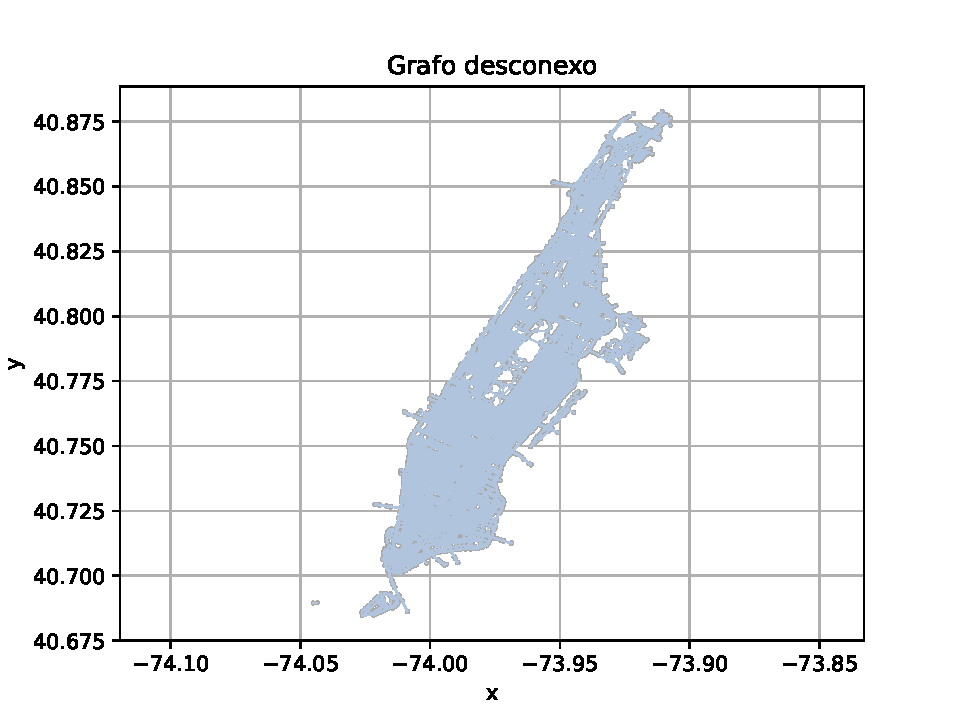
\includegraphics[width=0.6\textwidth, trim={0 .3cm 0 .9cm},clip]{../figs/fig1.pdf}
    \end{figure}

    \newpage

    \begin{figure}[ht]
        \centering
        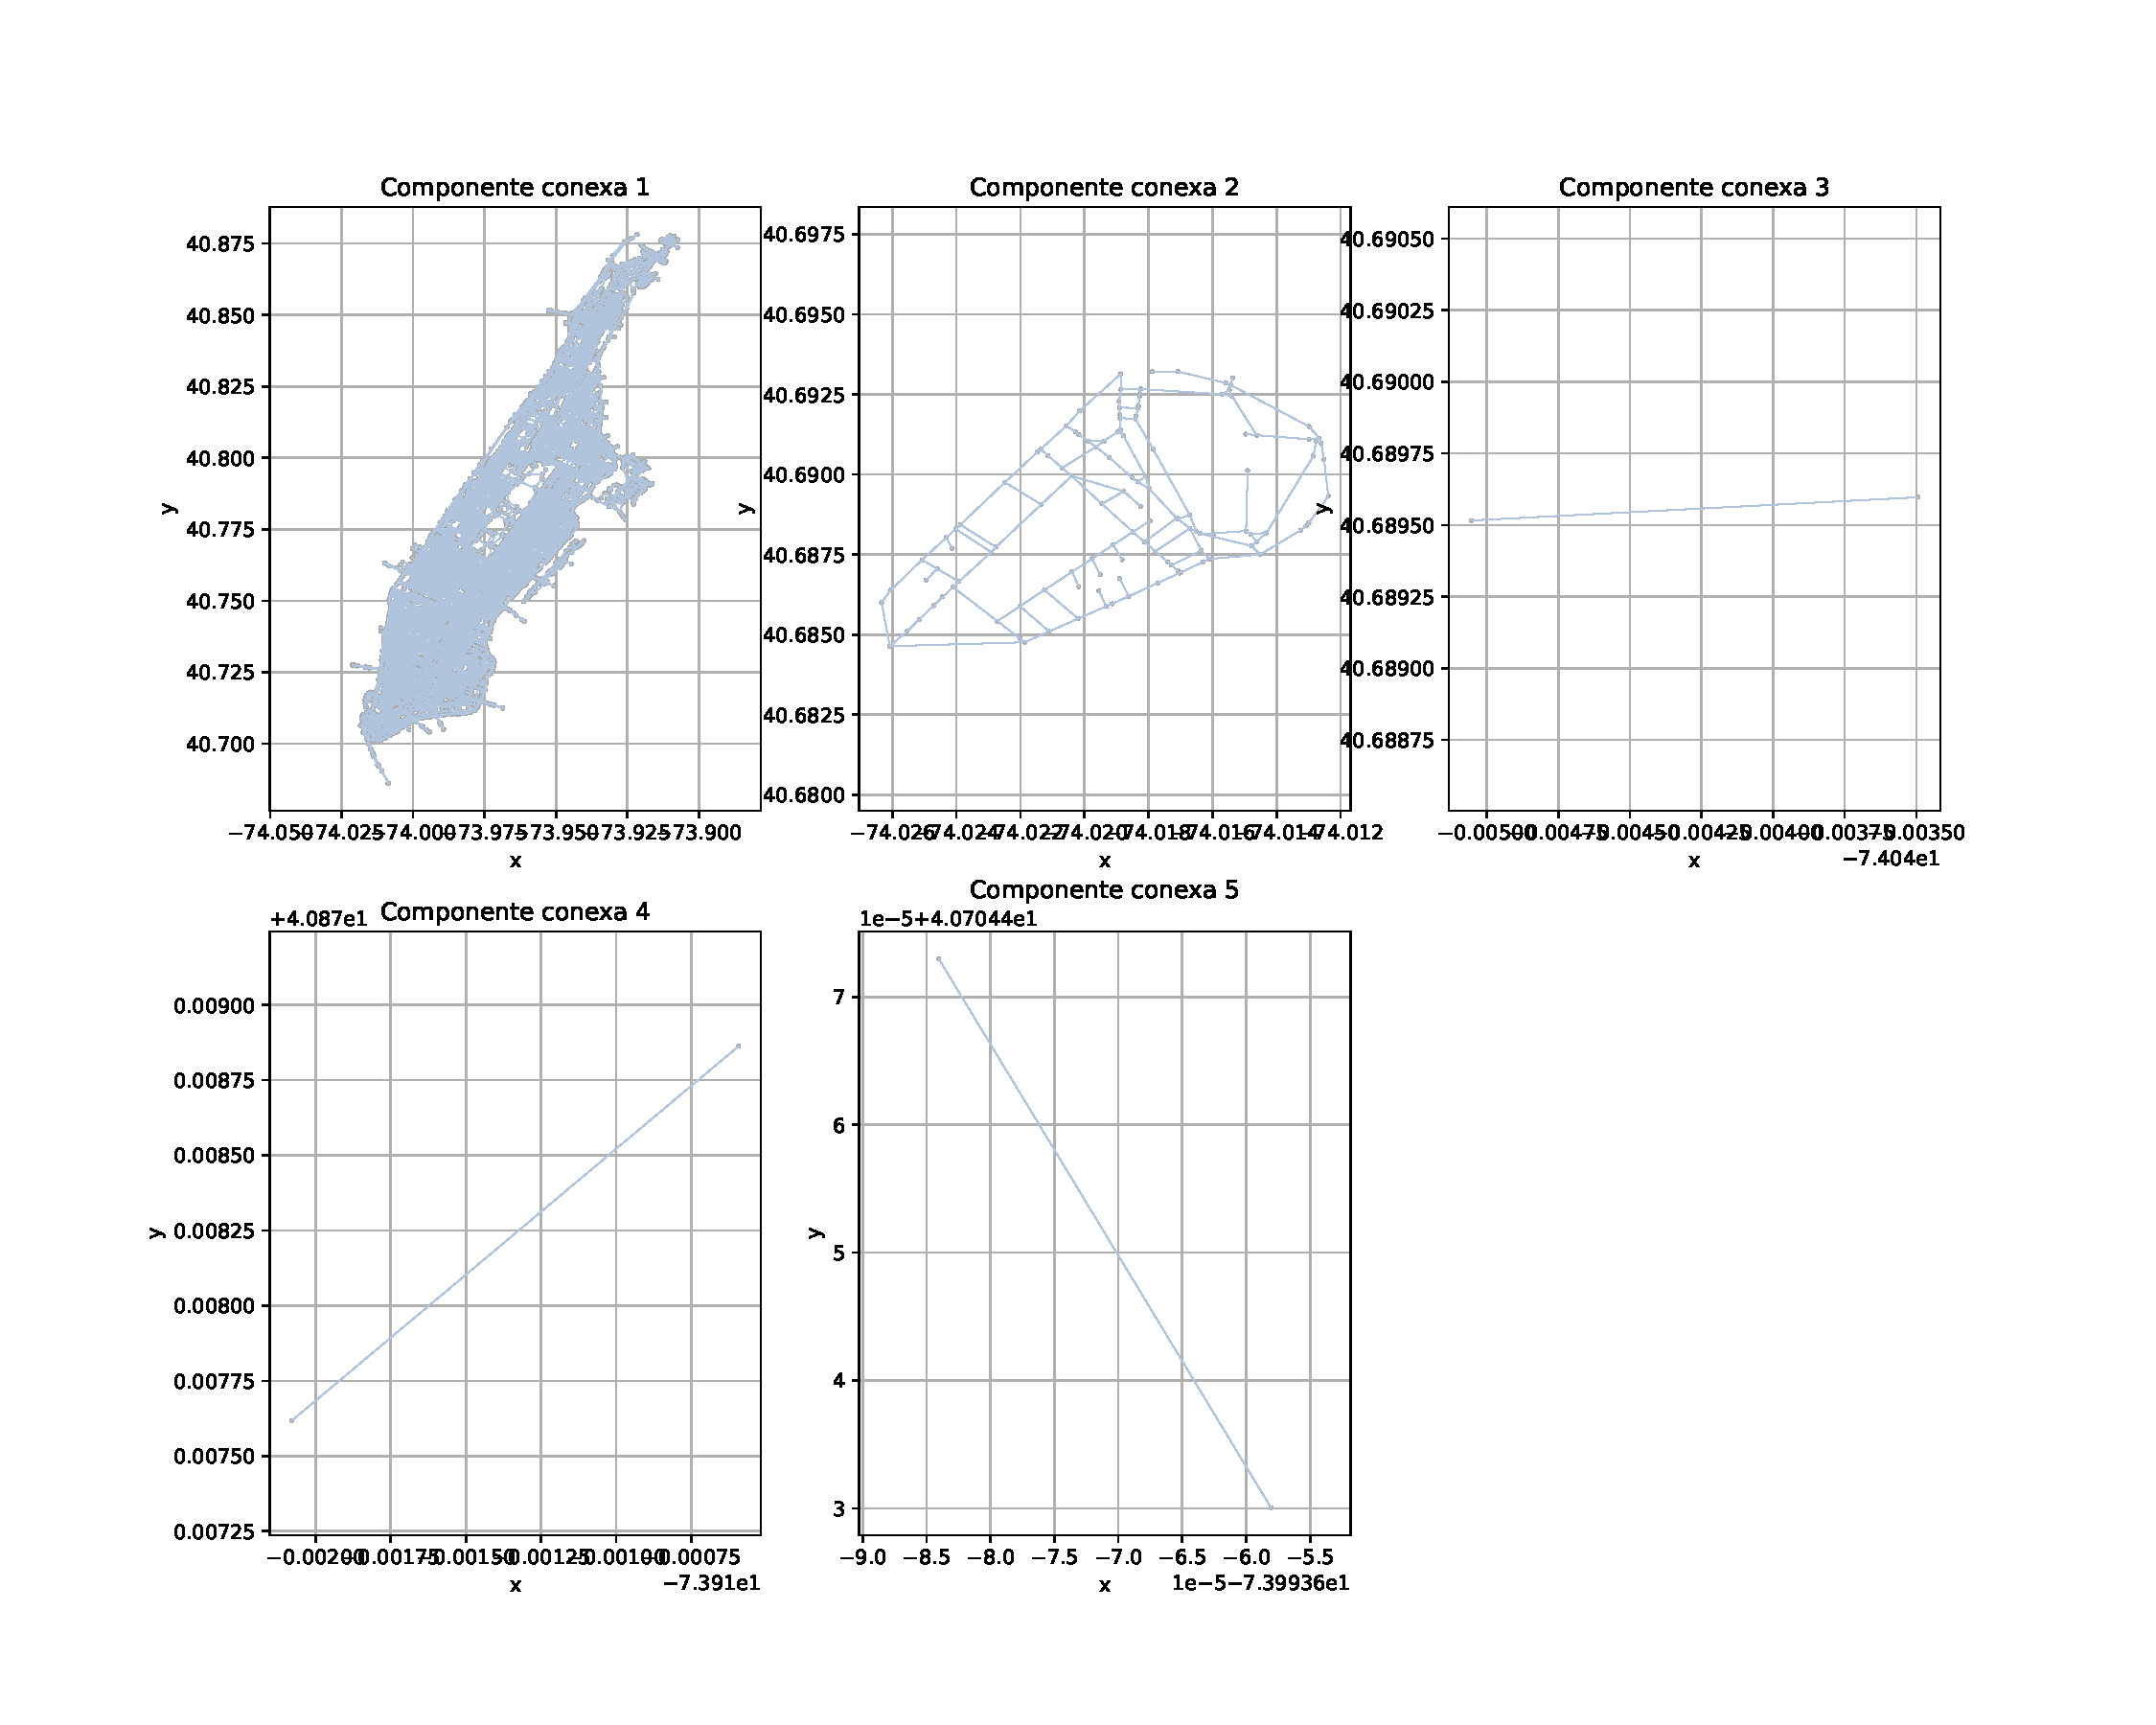
\includegraphics[width=0.9\textwidth, trim={0 2.3cm 0 3.1cm},clip]{../figs/fig2.pdf}
    \end{figure}

    \vspace{3cm}

    \begin{figure}[ht]
        \centering
        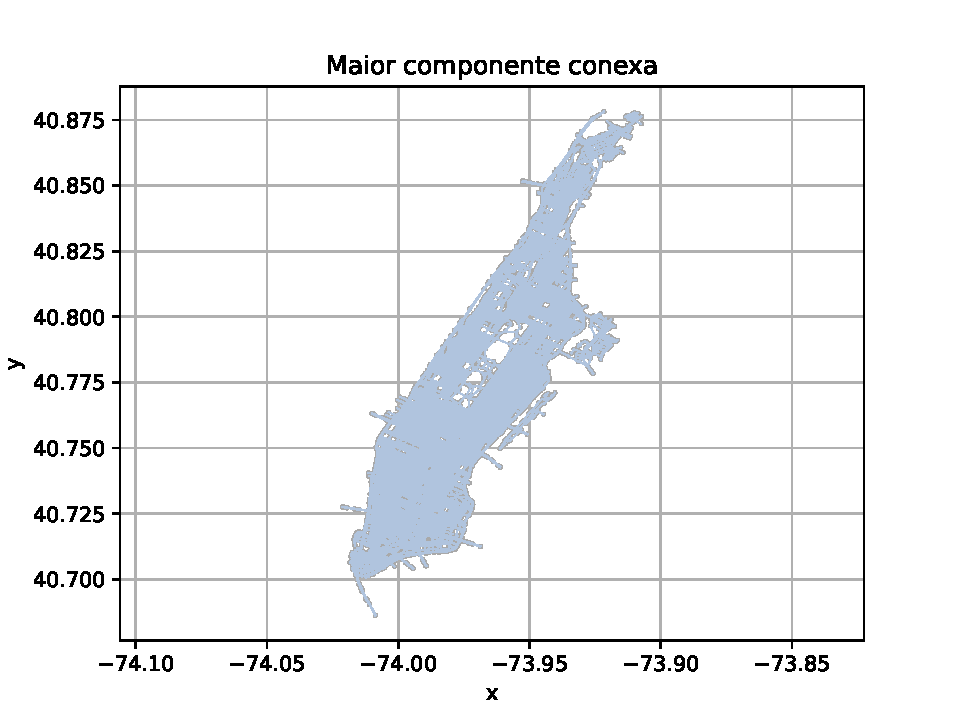
\includegraphics[width=0.64\textwidth, trim={0 10px 0 25px},clip]{../figs/fig3.pdf}
    \end{figure}

    \newpage

    \begin{figure}[ht]
        \centering
        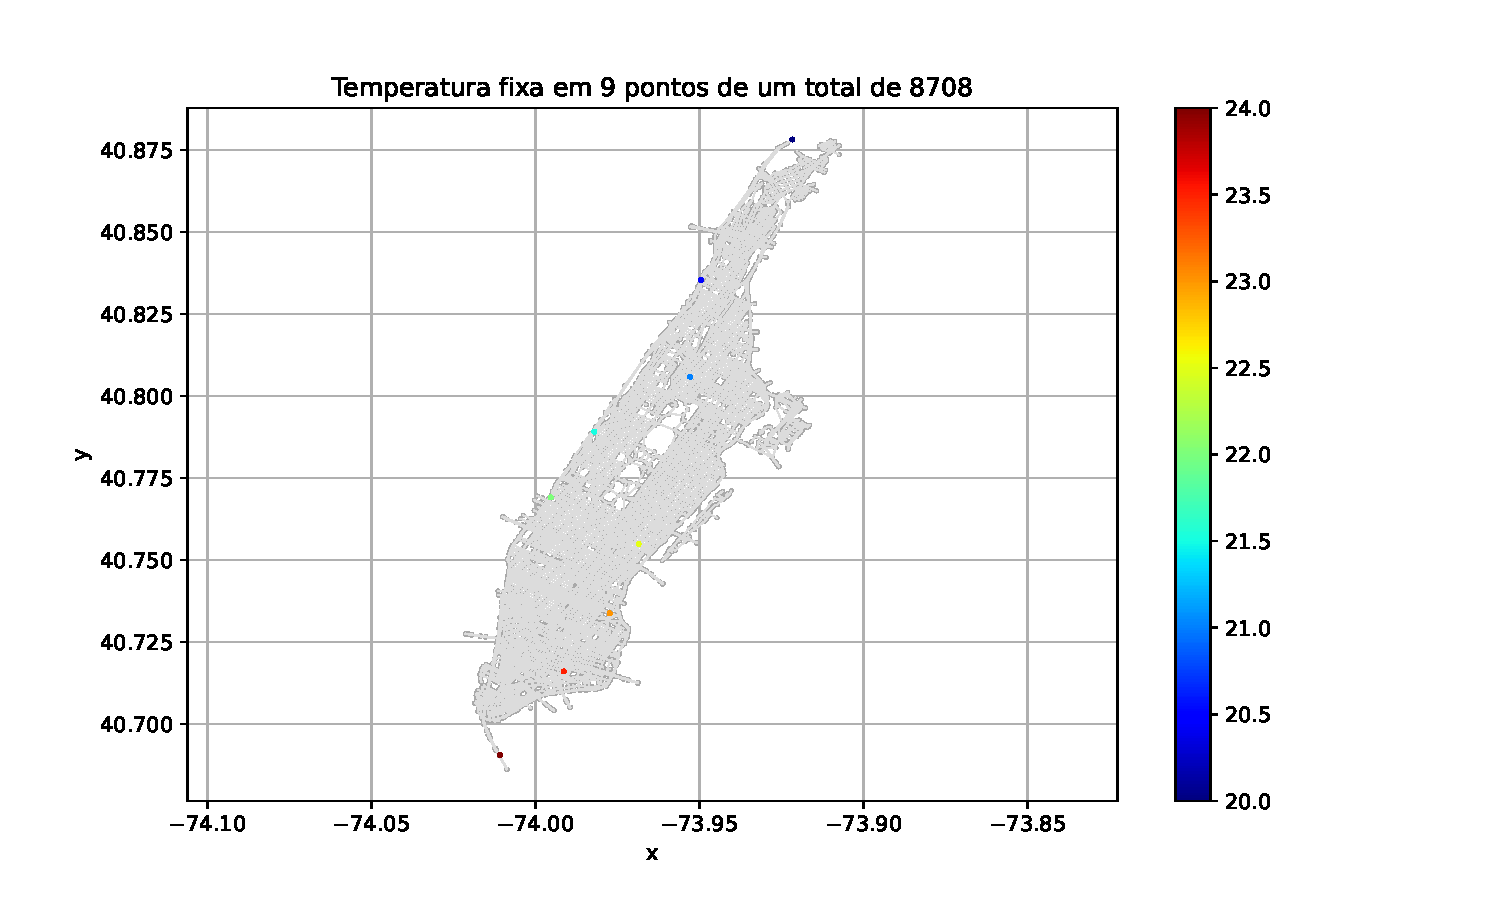
\includegraphics[width=0.7\textwidth, trim={0 10px 0 25px},clip]{../figs/fig4.pdf}
    \end{figure}

    \begin{figure}[ht]
        \centering
        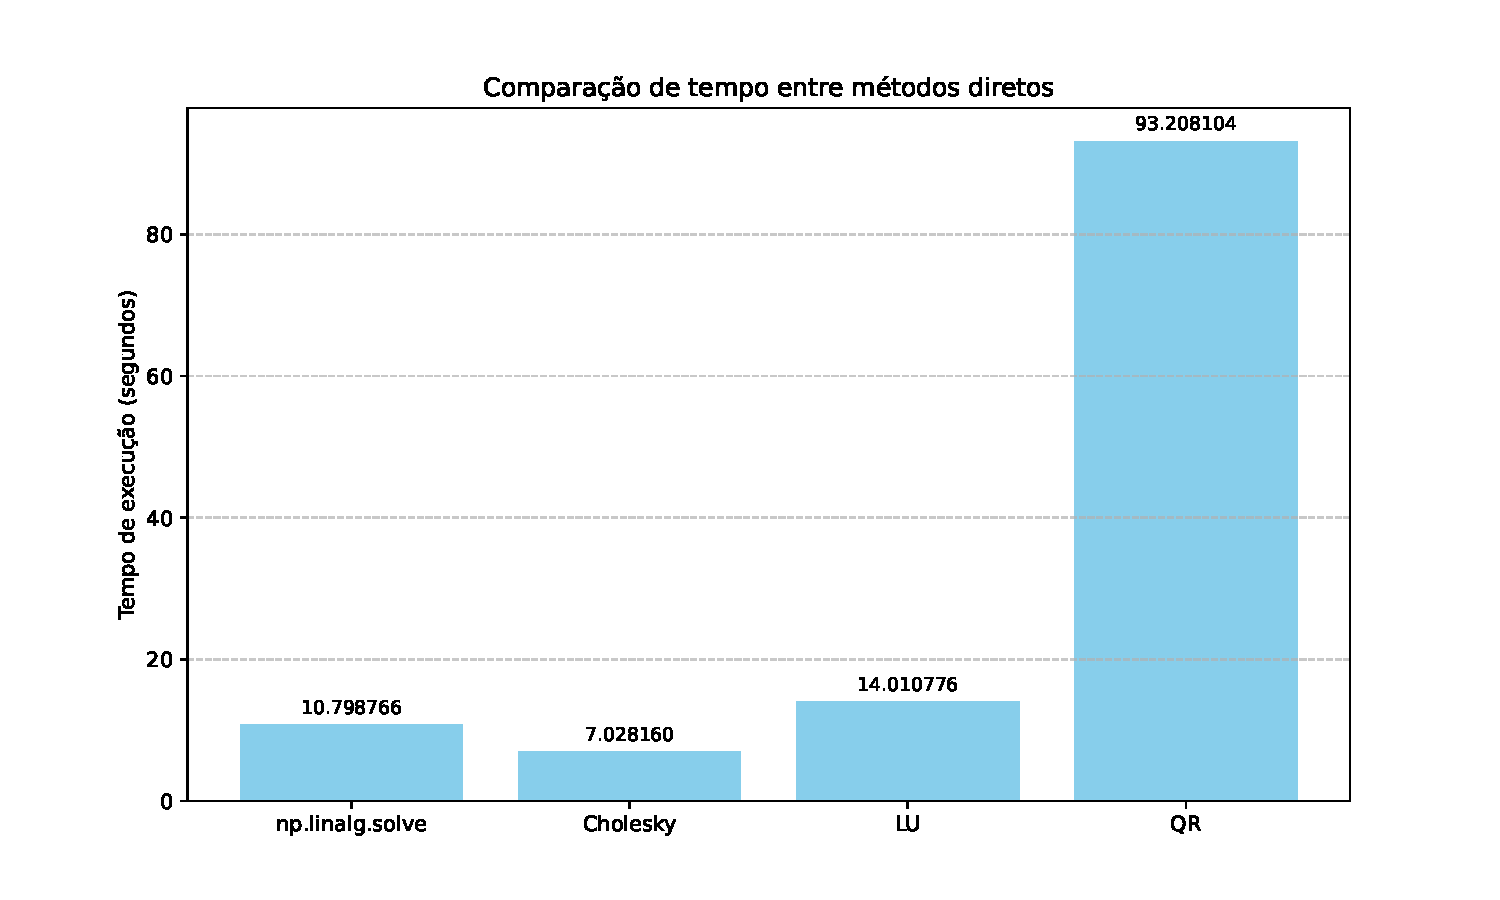
\includegraphics[width=1\textwidth, trim={0 10px 0 25px},clip]{../figs/fig5.pdf}
    \end{figure}

    \newpage

    \begin{figure}[ht]
        \centering
        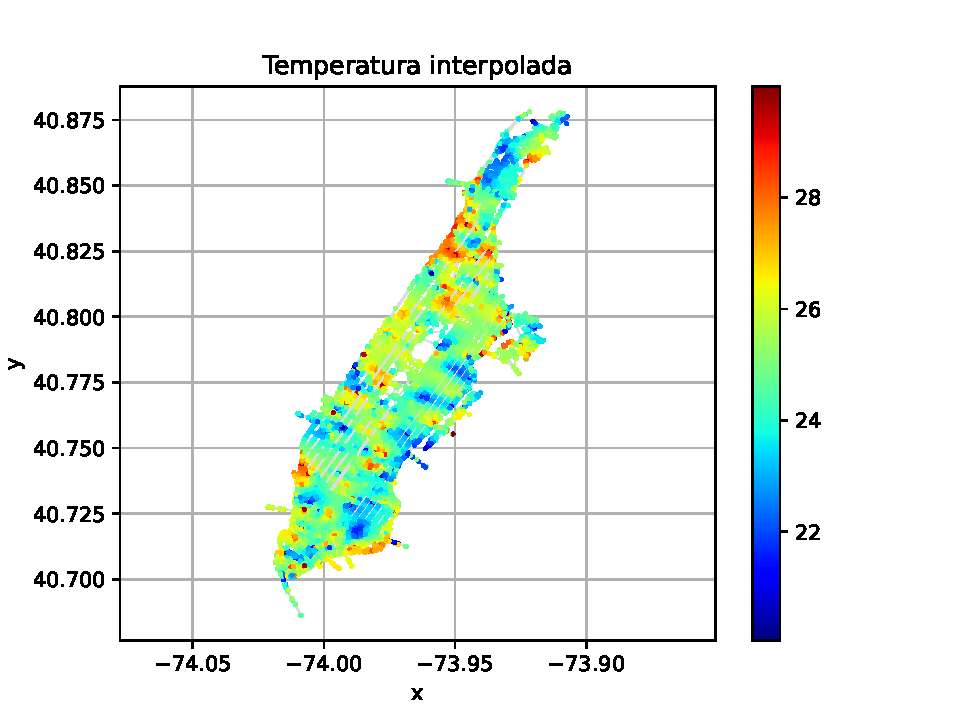
\includegraphics[width=0.7\textwidth, trim={0 10px 0 25px},clip]{../figs/fig6.pdf}
    \end{figure}

    \begin{figure}[ht]
        \centering
        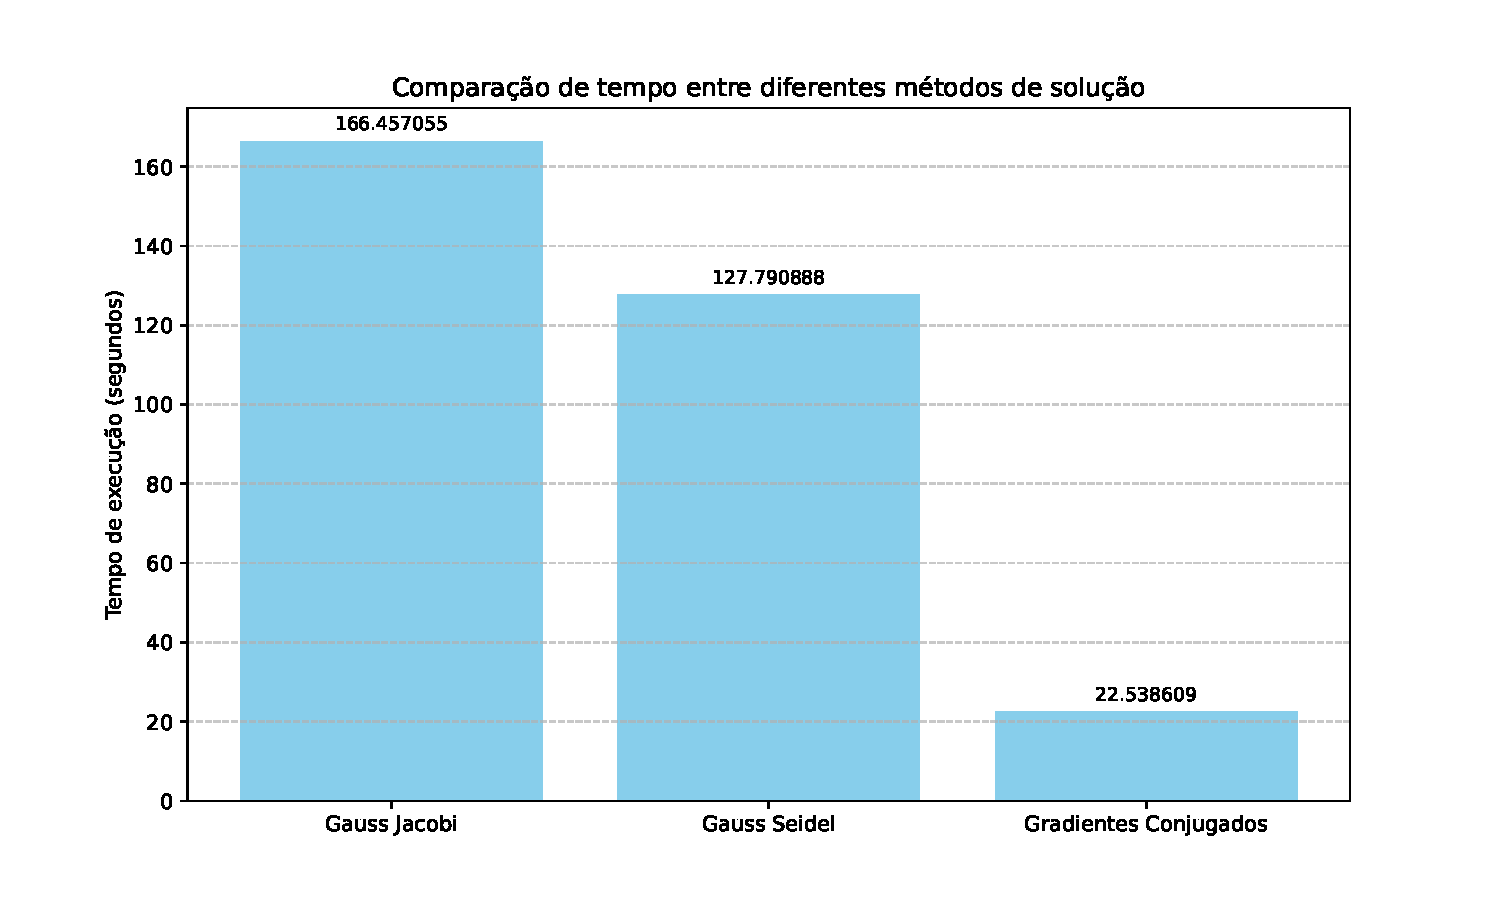
\includegraphics[width=1\textwidth, trim={0 10px 0 25px},clip]{../figs/fig7.pdf}
    \end{figure}
\end{document}